%% beamerthemeImperialPoster v1.0 2016/10/01
%% Beamer poster theme created for Imperial College by LianTze Lim (Overleaf)
%% LICENSE: LPPL 1.3
%%
%% This is the example poster demonstrating use
%% of the Imperial College Beamer Poster Theme
\documentclass[xcolor={table}]{beamer}
%% Possible paper sizes: a0, a0b, a1, a2, a3, a4 (although Imperial College posters are usually A0 or A1).
%% Possible orientations: portrait, landscape
%% Font sizes can be changed using the scale option.
\usepackage[size=a0,orientation=portrait,scale=1.55]{beamerposter}
\usepackage{amsmath}
\usetheme{ImperialPoster}
\usepackage{shorts}
\usepackage{lipsum}
% \usepackage{babel}
\usepackage{subfigure}
\usepackage{graphicx}
\usepackage[ampersand]{easylist}
%% Four available colour themes
\usecolortheme{ImperialWhite} % Default
\title{{\Large \textbf{Machine learning continuously monitored systems: estimating parameters}}}

\author{ {\normalsize Matías Bilkis, Giulio Gasbarri and John Calsamiglia  - Universitat Autònoma de Barcelona}}

\institute{}%Física Teòrica: Informació i Fenòmens Quàntics, Departament de Física,

\addbibresource{sample.bib}


\begin{document}
\begin{frame}[fragile=singleslide,t]\centering

\maketitle

\begin{columns}[onlytextwidth,T]

%%%% First Column
\begin{column}{.47\textwidth}

\begin{block}{Abstract}
  \parshape 1 0cm \dimexpr\linewidth-0cm\relax
  We consider the problem of estimating parameters that govern the dynamics of a continuously monitored system. To this end, we bring into stage the a recurrent cell which, aided with automatic differentiation, allows us to do maximum likelihood on the measurement signal; we compare estimation performance with respect to the ultimate attainable bound given by the Fisher information, and with Lorenztian fits of the spectral power. We next move on to machine-learning-estimate external controls' parameters. Doors and questions remain open to whether the presented approach can be useful to tackle sophisticated tasks, such as the identification of dynamical equations of motion out of measurement signals.
\end{block}

\begin{block}{The model}
  \parshape 1 0cm \dimexpr\linewidth-0cm\relax
We consider an optomechanical system under continuous homodyne detection on the optical mode, and in the Gaussian regime. The equations of motion read:
\begin{align}\label{eq:evo}
dx_t &= \big(A_\theta - \chi(\Sigma_t) C\big) x_t dt + \chi(\Sigma_t) dy = A_\theta x_t dt + \chi(\Sigma_t) dW_t \\
d\Sigma_t &= A_\theta \Sigma_t + \Sigma A_\theta^T + D - \chi(\Sigma_t)^T \chi(\Sigma_t) \nonumber¸\\
dy &= C(x_tdt + C^{-1}dW_t), \nonumber
\end{align}
where $(x_t,\Sigma_t)$ denote the first two moments of the mechanical mode at time $t$, and $dy_t$ denotes measurement outcome. Thus, the measurement model is Gaussian and centered on the value of the \textit{hidden state} $x_t$. The matrices and coefficients governing the dynamics read: {\normalsize$A = \Big(\;\begin{matrix}-\frac{\gamma}{2}& -\omega\\\omega & -\frac{\gamma}{2}\end{matrix}\;\Big), \; \; D = (\gamma (n + \frac{1}{2}) + \kappa )\mathbb{I}_2, \; \; C = \sqrt{\eta \kappa} \Big( \; \begin{matrix} 1 & 0 \\ 0 & 0 \end{matrix}\;\Big), \; \chi(\sigma) = \Sigma C^T $}
\end{block}
\begin{block}{Estimation}
  \parshape 1 0cm \dimexpr\linewidth-0cm\relax
  We focus on estimating the value of parameter $\theta$, appearing in Eq.~\eqref{eq:evo}. The log-likelihood $\lambda(y|\theta) = \log p(y|\theta)$ of getting a string of outcomes $y= (dy_0, ... dy_t)$ under $\theta$ can be computed through the measurement model, and in particular an evolution for the (derivative of ) the score $\partial^2_\theta \lambda(y|\theta)$ can be derived as
\begin{equation*}
d \partial^2_\theta \lambda = - |\partial_\theta C x| ^2 dt + (\partial_\theta^2 C x) dW_t,
\end{equation*}which in turn allows us to to numerically obtain the Fisher information $I[\theta] = \sum_t \mathbb{E}[|\partial_\theta C x|^2] dt$. This quantity lower bounds the variance of any unbiased estimation $\hat{\theta}$.

Here, we propose a recurrent unit which computes $\hat{\theta} = \text{argmax}\lambda(y|\hat{x}_{\hat{\theta}})$ where $\hat{x}_{\hat{\theta}}$ \textit{tracks} the hidden state in ressemblance to Kalman filters. As an example, we consider estimating the mechanical mode's frequency $\omega$, appearning in $A$ matrix in Eq~\eqref{eq:evo}. We compare recurrent unit performance with  Lorentzian fits over the spectral power and the Fisher information.

\end{block}

\begin{figure}
\centering
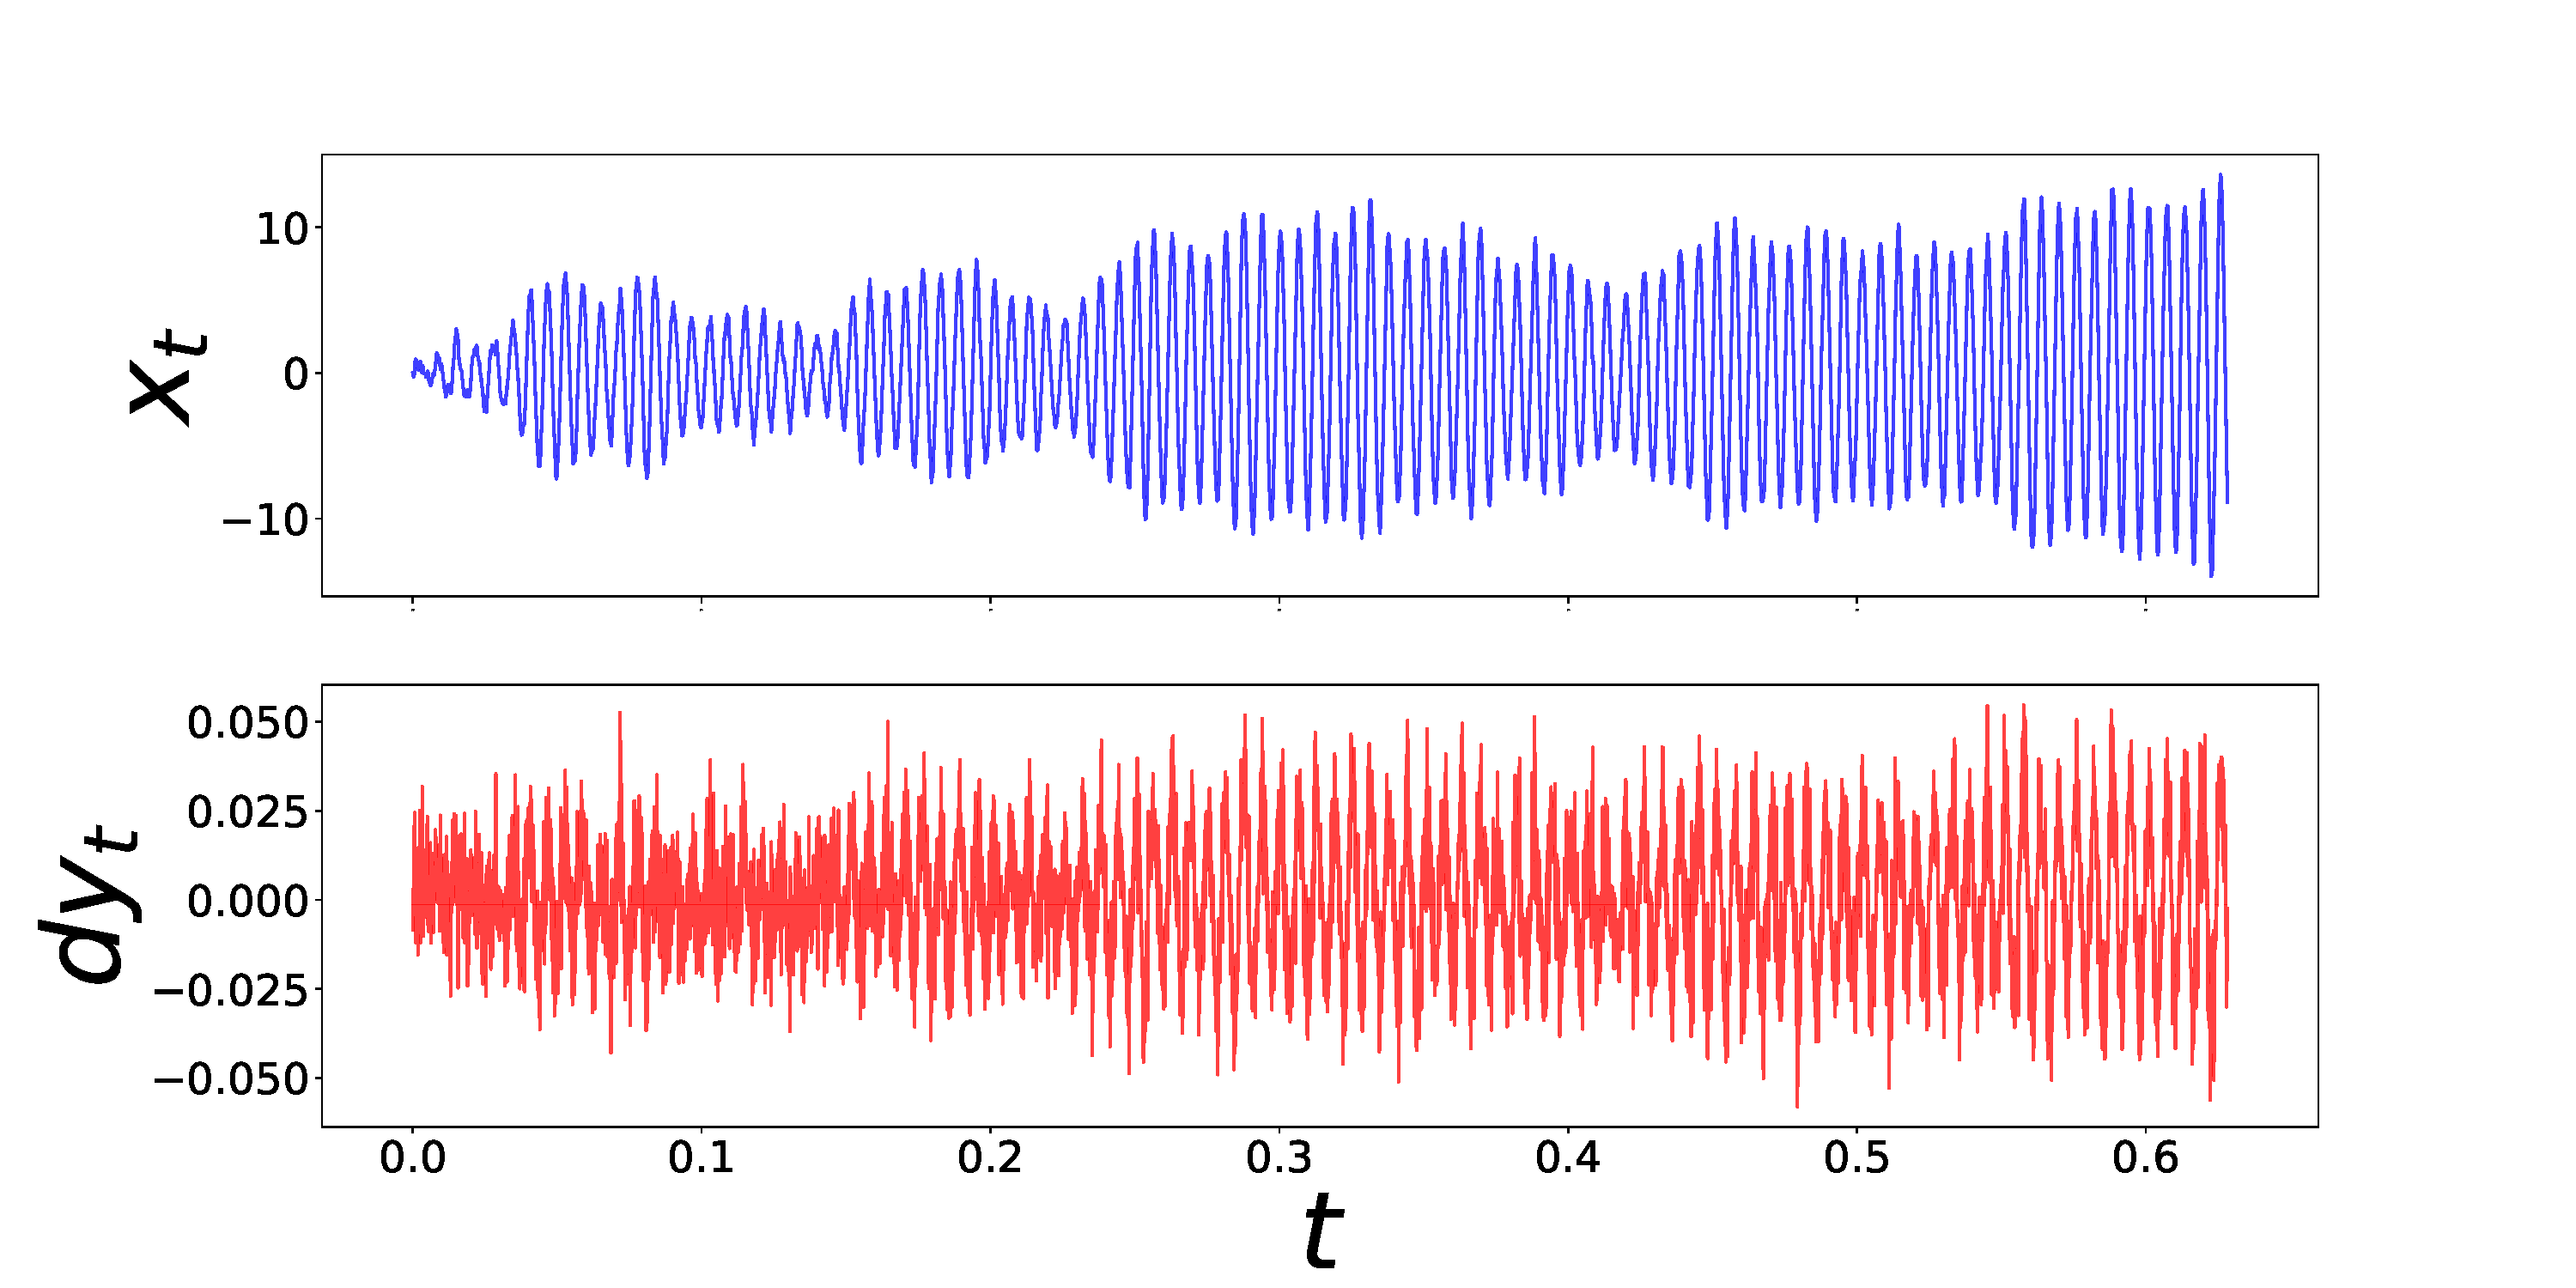
\includegraphics[width=.49\hsize]{figures_poster/evolution.pdf}
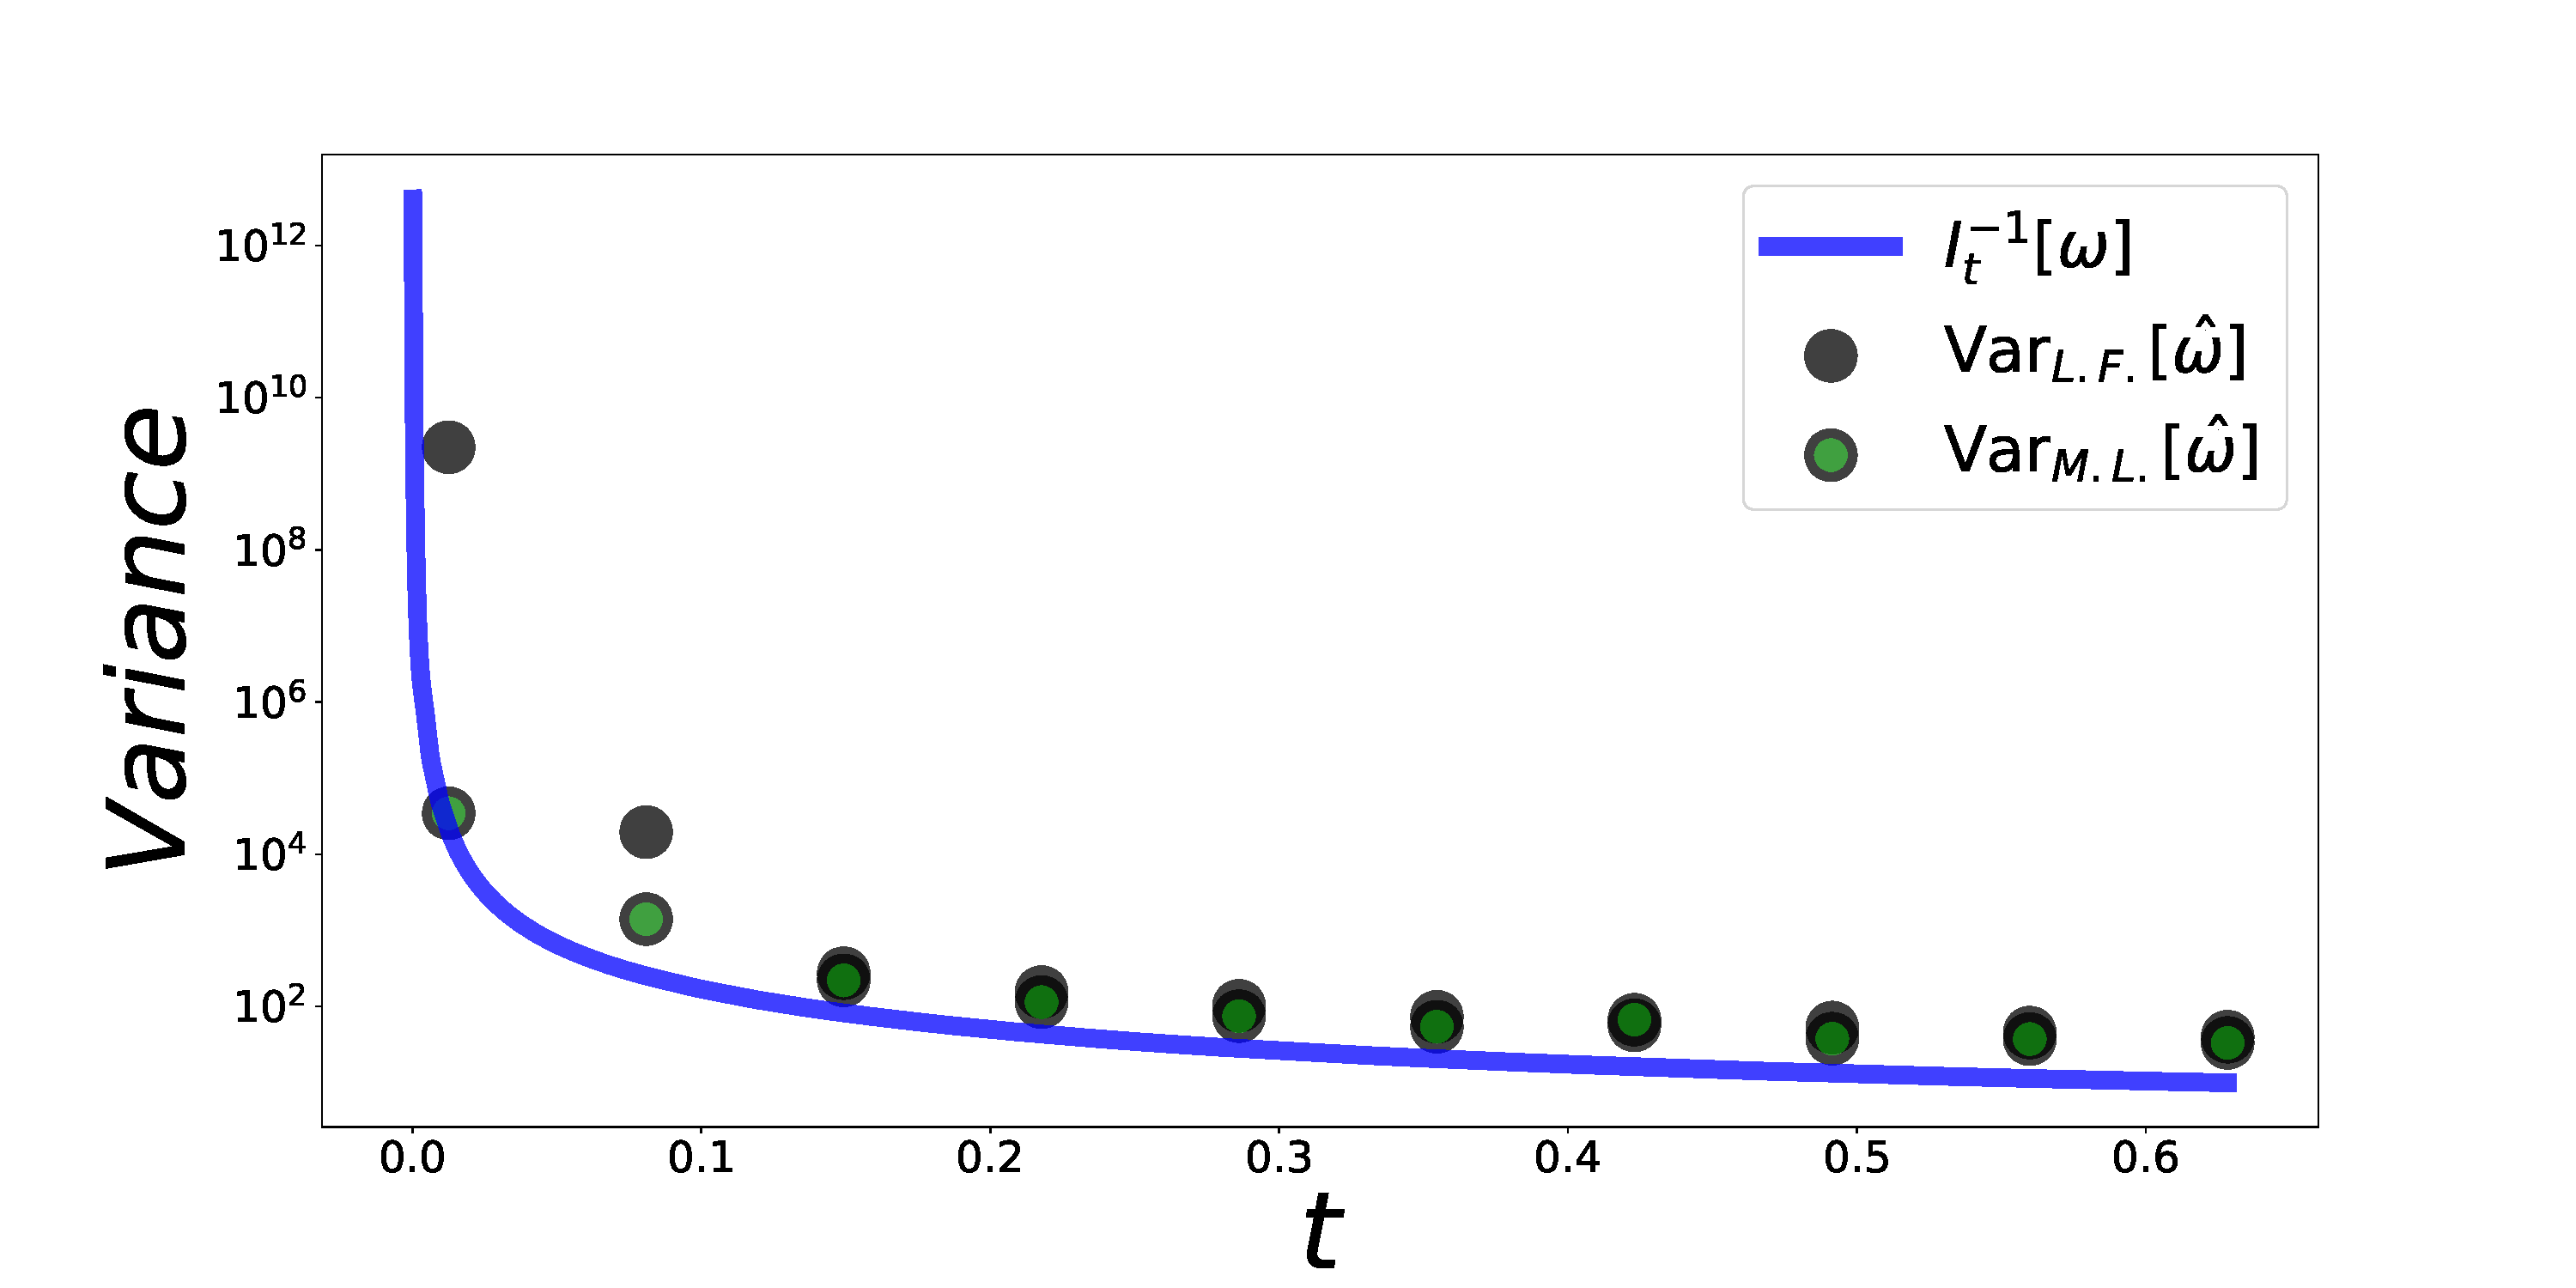
\includegraphics[width=.49\hsize]{figures_poster/variance_comparison_hori.pdf}

\vspace{1cm}

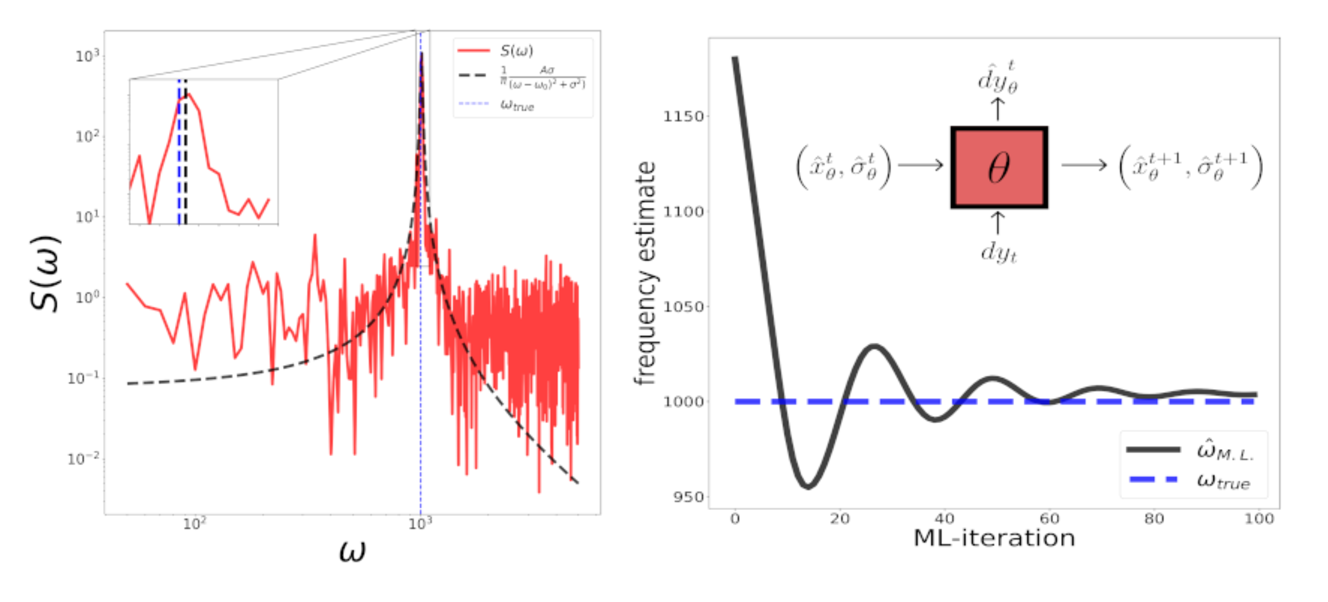
\includegraphics[width=1.\hsize]{figures_poster/dos.pdf}}
\end{figure}
\vspace{2cm}
\end{column}

%%%% Second Column
\begin{column}{.47\textwidth}
\begin{block}{External controls}
  Signals for the cavity surroundings $f^t_\theta$, such as forces, can be included in the evolution Eq.~\eqref{eq:evo} as per:
  \begin{align}
  dx_t &= \big(A_\theta - \chi(\Sigma_t) C\big) x_t dt + \chi(\Sigma_t) dy + f^t_\theta dt
  \end{align}
  While the structure of the external signal might potentially be complicated, we test our machine-learning machinery in the case of \textit{(i)} constant force, \textit{e.g.} $f^t_\theta = f$ , and \textit{(ii)} eponentially damped force \textit{e.g.} $f^t_\theta = A e^{-t/\tau}$. Here, the task is to estimate $f$ and $(A, \tau)$ respectively out of measurement signal $dy_t$.
{\center
\begin{figure}
\centering
  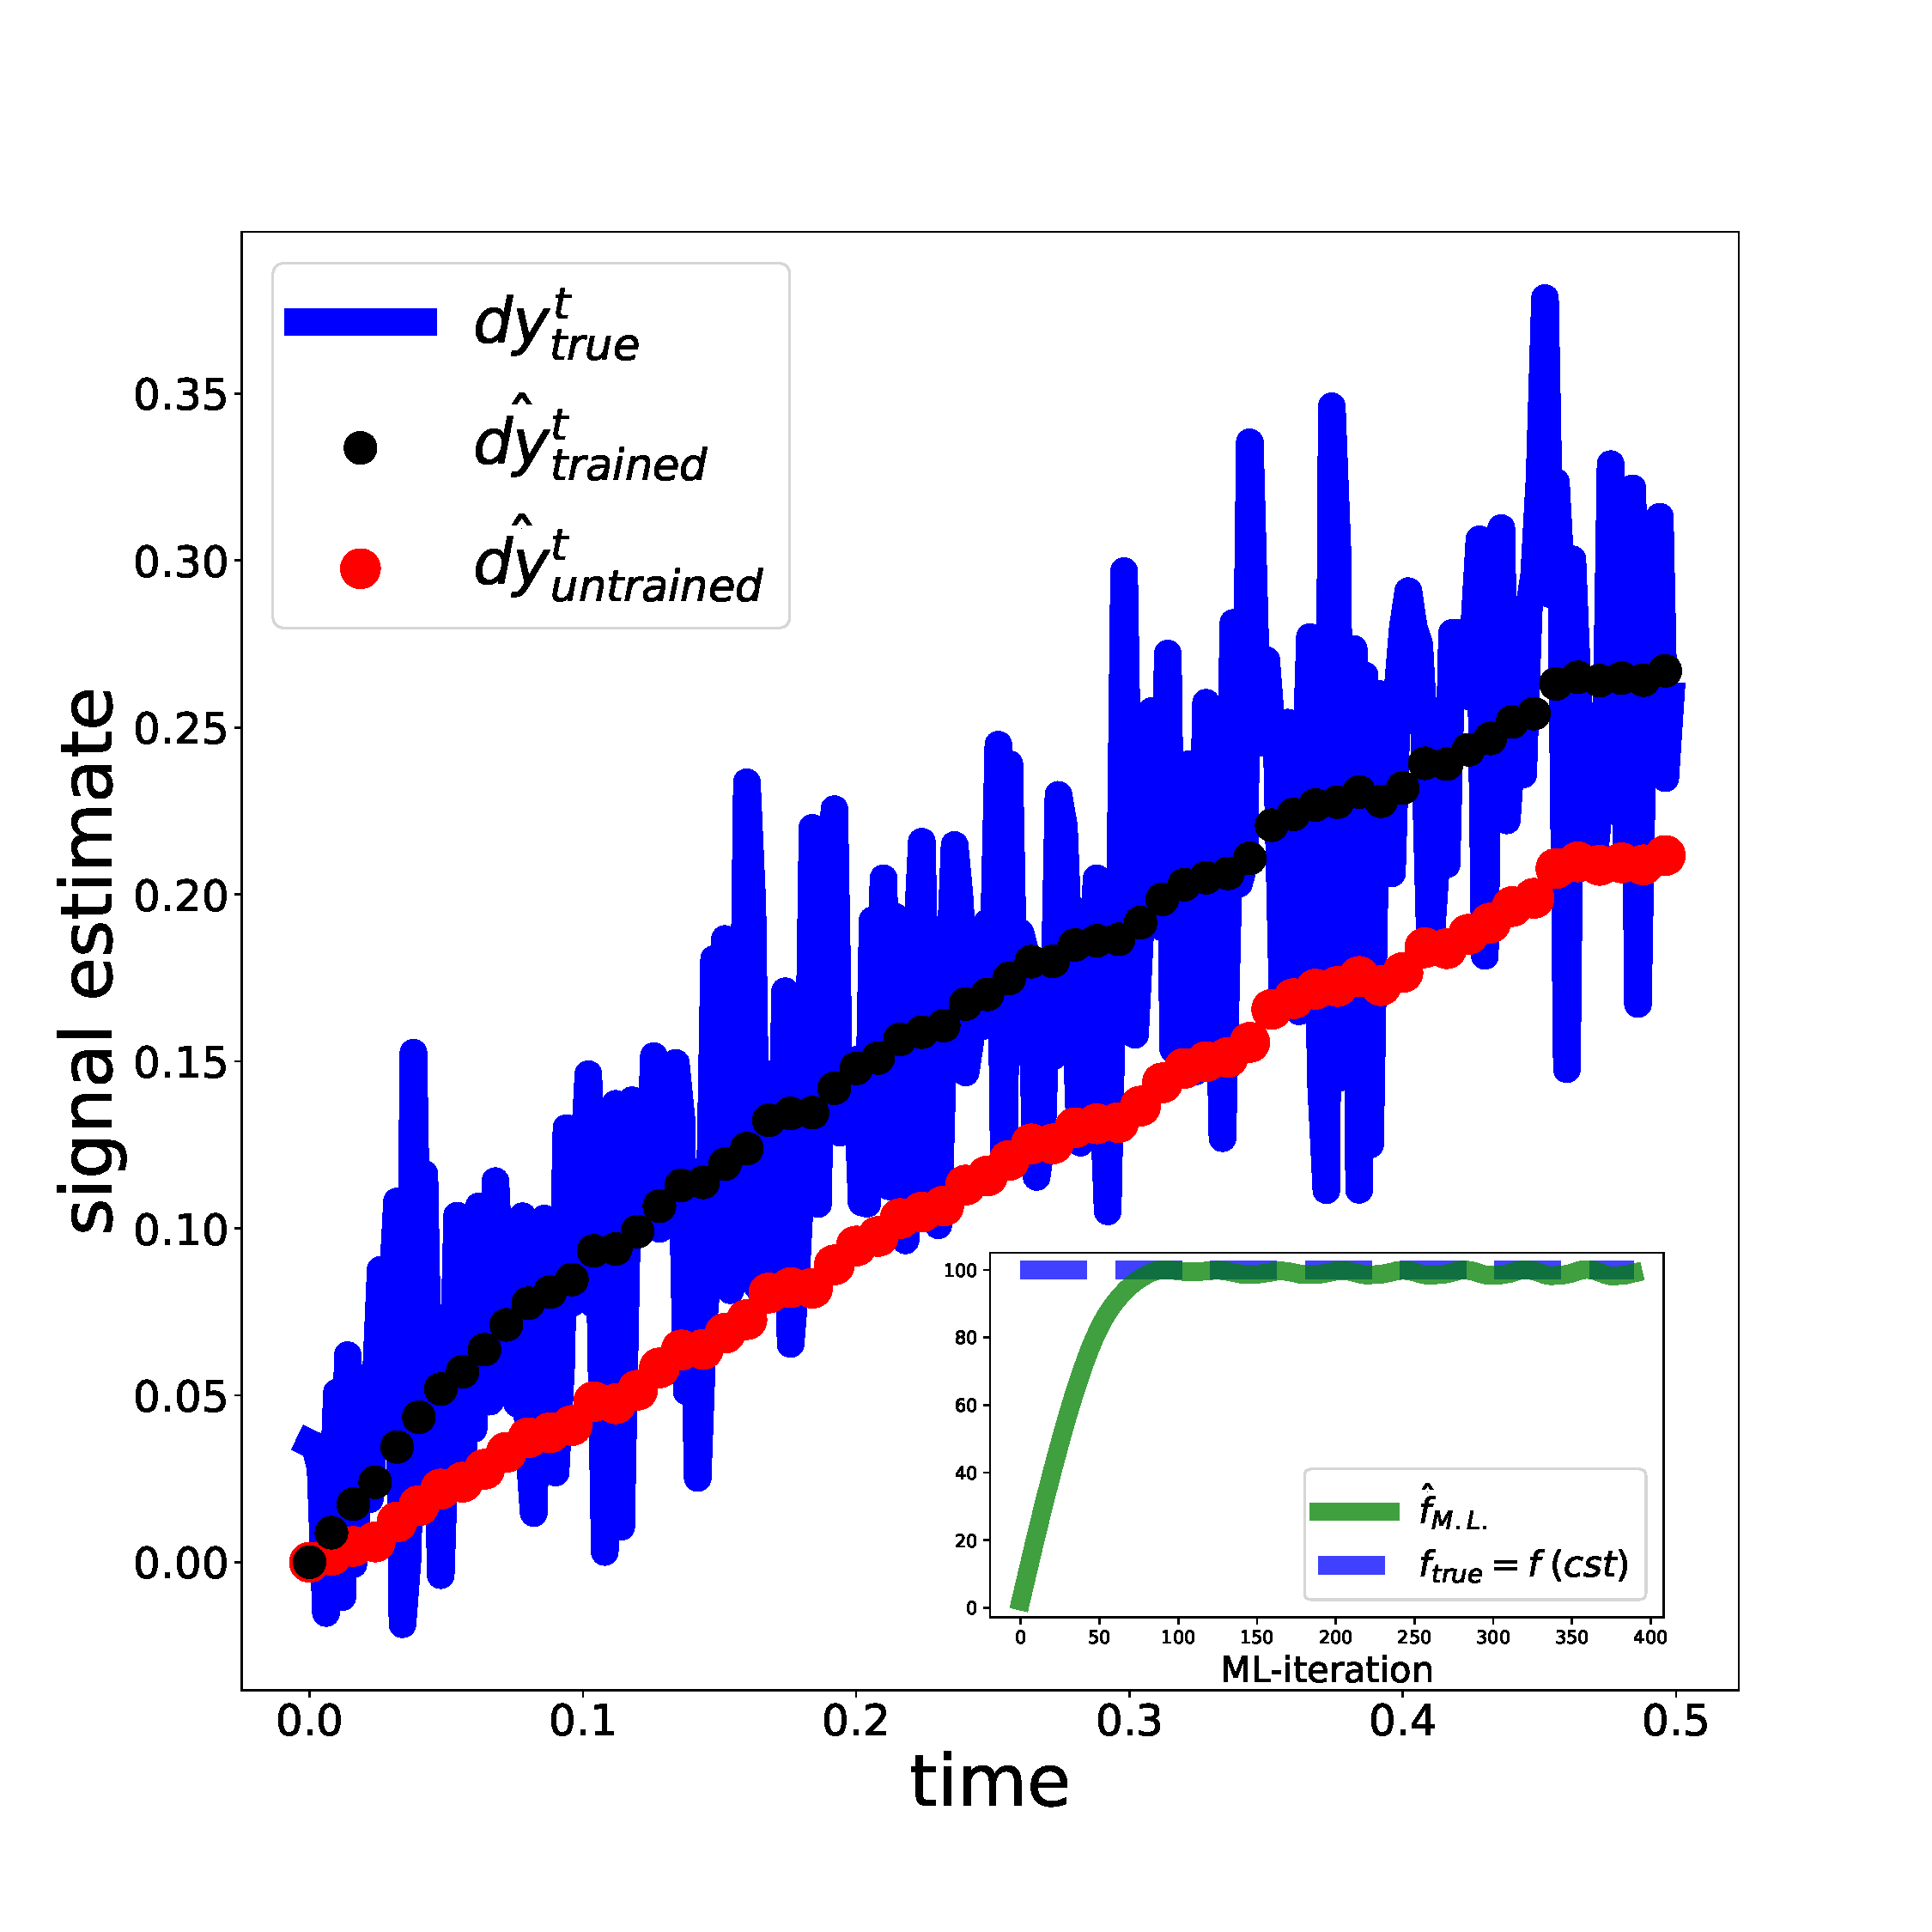
\includegraphics[width=.9\textwidth]{figures_poster/external_learn_signals.pdf}
  \centering
  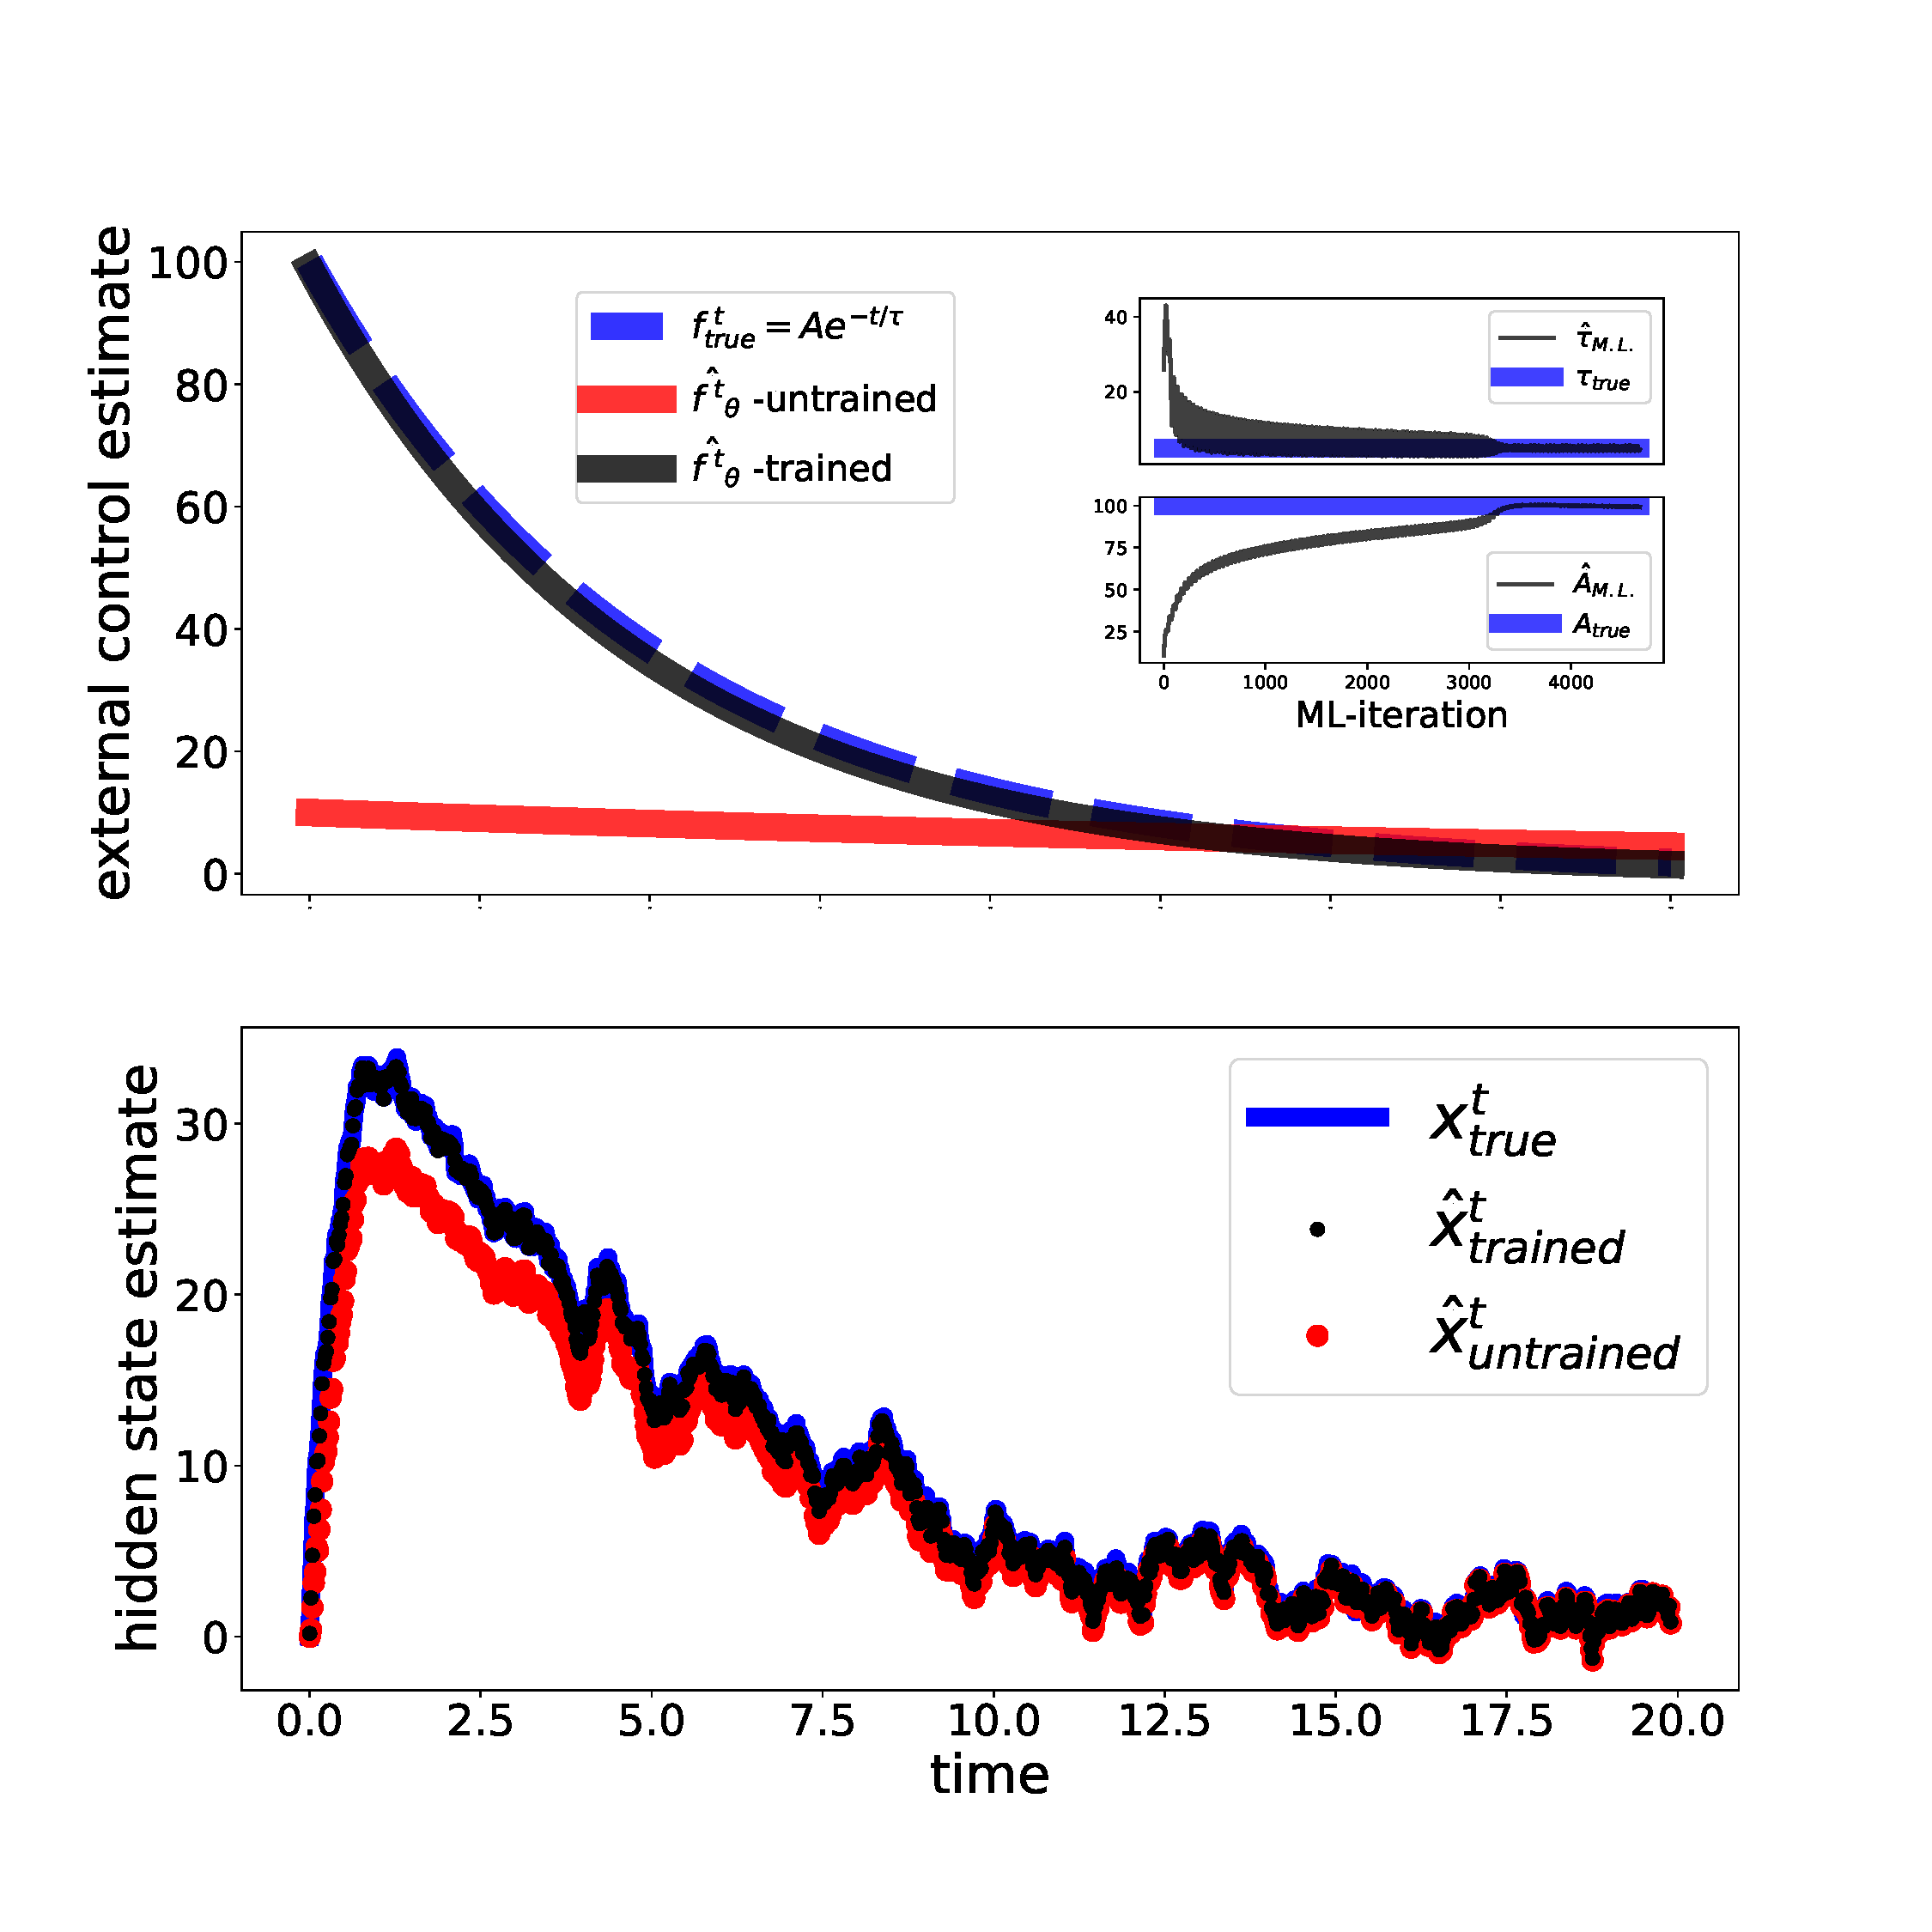
\includegraphics[width=.9\textwidth]{figures_poster/external_learn_track_example2.pdf}
  }
\end{figure}

\end{block}


\begin{block}{Conclusion}
  We introduced a machine-learning method which is able to track the hidden state out of measurement data, and thorugh the internal model make an estimation of hidden Markov dynamics (and in particular of the parameters value). Among interesting directions are those of inferring dynamical equations out of measurement data, in cases where $f_\theta^t$ has a more sophisticated structure.
  \end{block}


\begin{block}{Code}

\includegraphics[width=.15\textwidth]{figures_poster/qr_repo.pdf}
\end{block}


\printbibliography

\end{column}
\end{columns}


\end{frame}
\end{document}
